% !TeX spellcheck = sk_SK-Slovak
\documentclass[slovak]{beamer}
% \documentclass[slovak, handout]{beamer}
\usepackage{newalg, wasysym, slashbox,lscape}
\usepackage{multirow}
\usepackage{multimedia}
\usepackage[normalem]{ulem}
%\usepackage{hyperref}
\usepackage{graphicx}
\usepackage{booktabs}
\usepackage{hhline}
\usepackage{xcolor}

\newcommand\coloreditem[1]{\item[\textcolor{#1}{\usebeamertemplate{itemize \beameritemnestingprefix item}}]}

\mode<presentation>
{
  \usetheme{Goettingen}
}

\usepackage{babel}
\usepackage[utf8]{inputenc}
%\usepackage[english]{babel}
% or whatever

%\usepackage[latin1]{inputenc}
% or whatever

\usepackage{times}
\usepackage[T1]{fontenc}
% Or whatever. Note that the encoding and the font should match. If T1
% does not look nice, try deleting the line with the fontenc.

\setbeamertemplate{headline}{\vskip10pt}
\setbeamertemplate{frametitle}{\insertframetitle\par\vskip-10pt}

%\usepackage{epsfig}
%\usepackage{pgf,pgfarrows,pgfnodes,pgfautomata,pgfheaps}

\title[Predikcia budúcich nákladov na pacienta]{Predikcia budúcich nákladov na pacienta}


\author[]{Marián Kravec \\ školiteľ: MSc. František Dráček }

\date{}

%\institute[]{Katedra Aplikovanej Informatiky\\ Fakulta Matematiky, Fyziky a Informatiky \\Univerzita Komensk\'eho}



% If you have a file called "university-logo-filename.xxx", where xxx
% is a graphic format that can be processed by latex or pdflatex,
% resp., then you can add a logo as follows:

% \pgfdeclareimage[height=0.5cm]{university-logo}{university-logo-filename}
% \logo{\pgfuseimage{university-logo}}

% Delete this, if you do not want the table of contents to pop up at
% the beginning of each subsection:
\AtBeginSection[]
{
  \begin{frame}<beamer>
    \frametitle{Obsah}
    \tableofcontents[currentsection,currentsubsection]
  \end{frame}
}


% If you wish to uncover everything in a step-wise fashion, uncomment
% the following command:

%\beamerdefaultoverlayspecification{<+->}
\beamerdefaultoverlayspecification{<+->}

% \newtheorem{Vysl}[theorem]{V�sledok}
% \newtheorem{Idea}[theorem]{My�lienka}

\def\ang#1{}

\begin{document}

\begin{frame}
  \titlepage
\end{frame}


% Since this a solution template for a generic talk, very little can
% be said about how it should be structured. However, the talk length
% of between 15min and 45min and the theme suggest that you stick to
% the following rules:

% - Exactly two or three sections (other than the summary).
% - At *most* three subsections per section.
% - Talk about 30s to 2min per frame. So there should be between about
%   15 and 30 frames, all told.

\section{Cieľ práce}

%\subsection{Problém Univerzitnej nemocnice}
\begin{frame}
  \frametitle{Cieľ práce}
	Predikovanie budúcej nákladovej skupiny do ktorej bude pacient v budúcnosti patriť na základe jeho minulosti a súčasného zdravotného stavu 
\end{frame}


\section{Dáta}

\begin{frame}  
	\frametitle{Dáta}
	\begin{itemize}
		\item<1> Zdroj dát: NCZI
		\item<1> Typ dát: poistné dáta
		\item<1> Jeden záznam: informácia o jednom výkone/lieku konkrétneho pacienta
		\item<1> Datasety:
		\begin{itemize}
			\item<1> Dataset ambulantnej zdravotnej starostlivosti 
			\item<1> Dataset ústavnej zdravotnej starostlivosti
			\item<1> Dataset predpísaných liekov
		\end{itemize}
		\item<1> V súčastnosti využívaná malá anonymizovaná vzorka
	\end{itemize} 
\end{frame}

\begin{frame}  
	\frametitle{Najdôležitejšie údaje pre časový rad}
	\begin{itemize}
		\item<1> Čas od prvého výkonu
		\item<1> Vek pacienta
		\item<1> Medicínsky výkon
		\item<1> Diagnóza
		\item<1> Liek 
		\item<1> Cena výkonu/lieku
	\end{itemize} 
\end{frame}

\section{Embedding}

\subsection{Výkony}

\begin{frame}
	\frametitle{Výkony}
	\begin{itemize}
		\item<1> Language-agnostic BERT sentence embedding model (LaBSE)
	\end{itemize}
		
	\begin{center}
		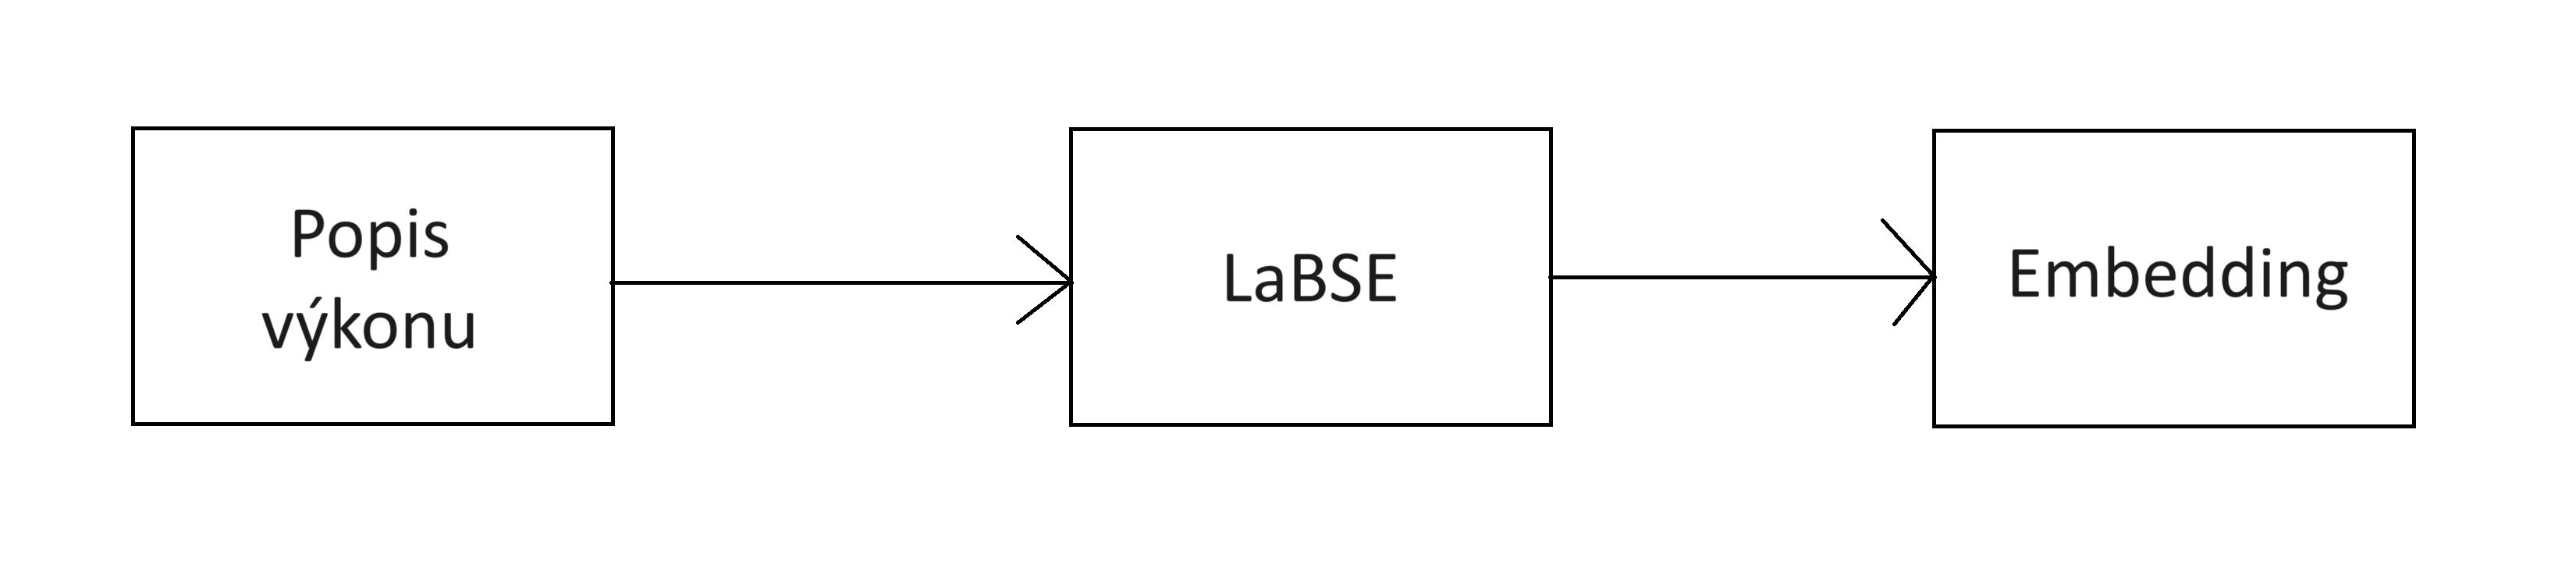
\includegraphics[height=2cm]{images/LaBSE.png}
	\end{center}
	
	\begin{itemize}
		\item<1> Lemmatizer + Word2vec model
	\end{itemize}
	
	\begin{center}
		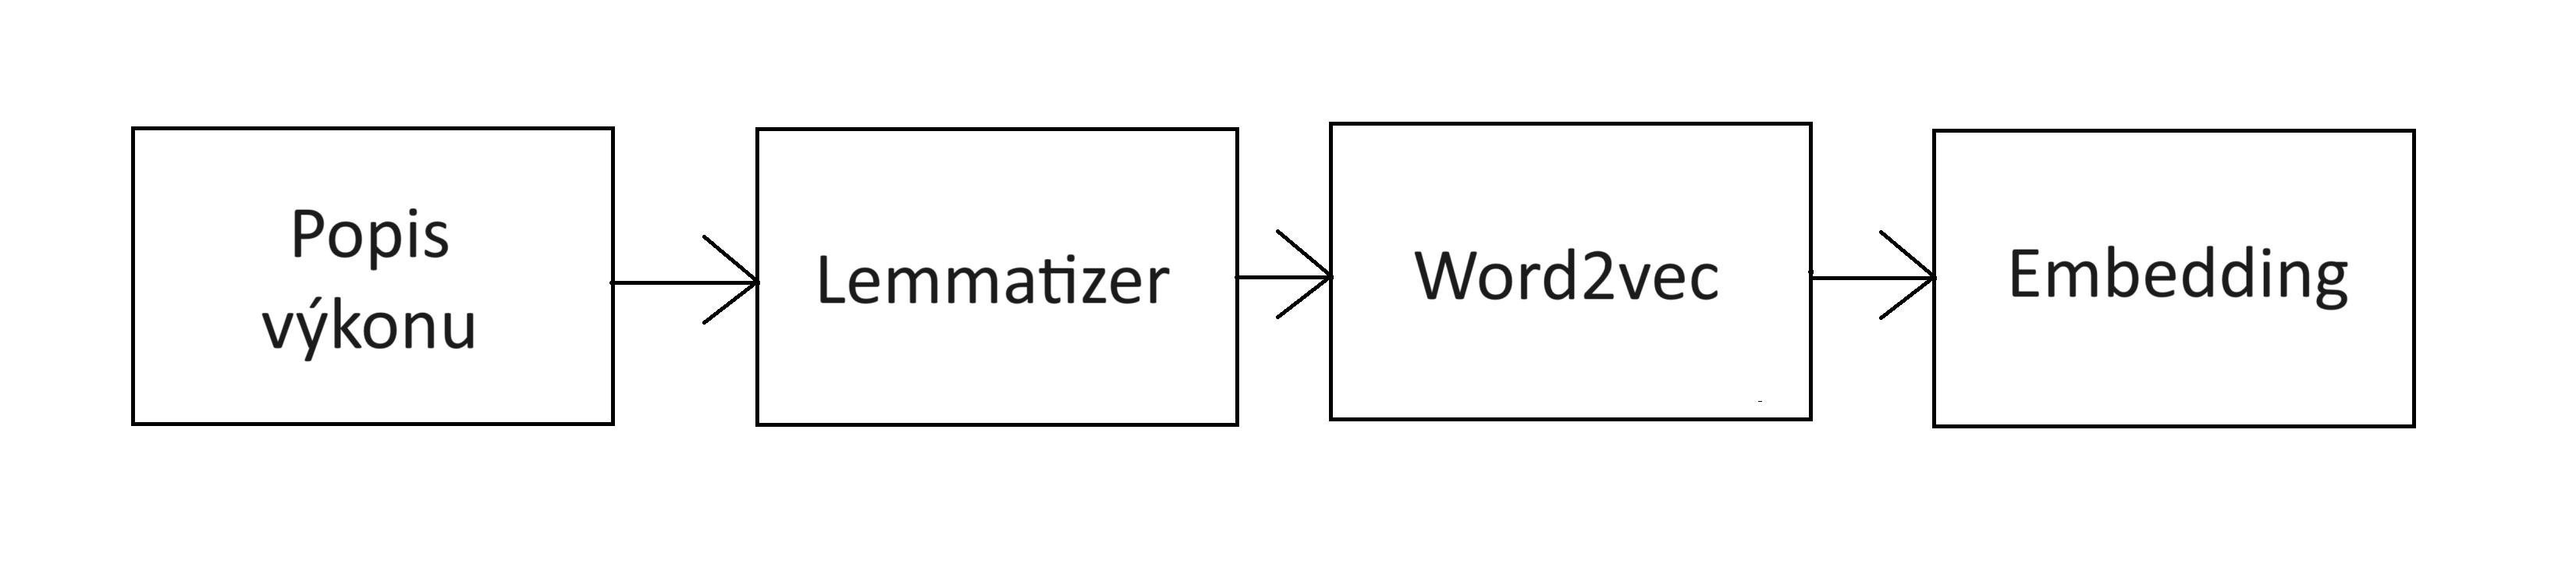
\includegraphics[height=2cm]{images/LemW2v.png}
	\end{center}
\end{frame}

\subsection{Diagnózy}

\begin{frame}
	\frametitle{Diagnózy}
	\begin{itemize}
		\item<1> ICD-10-CM kódy
	\end{itemize}

	\begin{center}
		
\includegraphics[height=0.7cm]{images/ICD_code.png}
	\end{center}
	\begin{itemize}
		\item<1> J - Choroby dýchacej sústavy
		\item<1> J3 - Iné choroby dýchacích ciest 
		\item<1> J38 - Choroba hlasiviek a hrtana
		\item<1> J38.0 - Obrna hlasiviek a hrtana
		\item<1> J38.01 - Jednostranná čiastočná obrna hlasiviek a hrtana
	\end{itemize}

	\begin{center}
		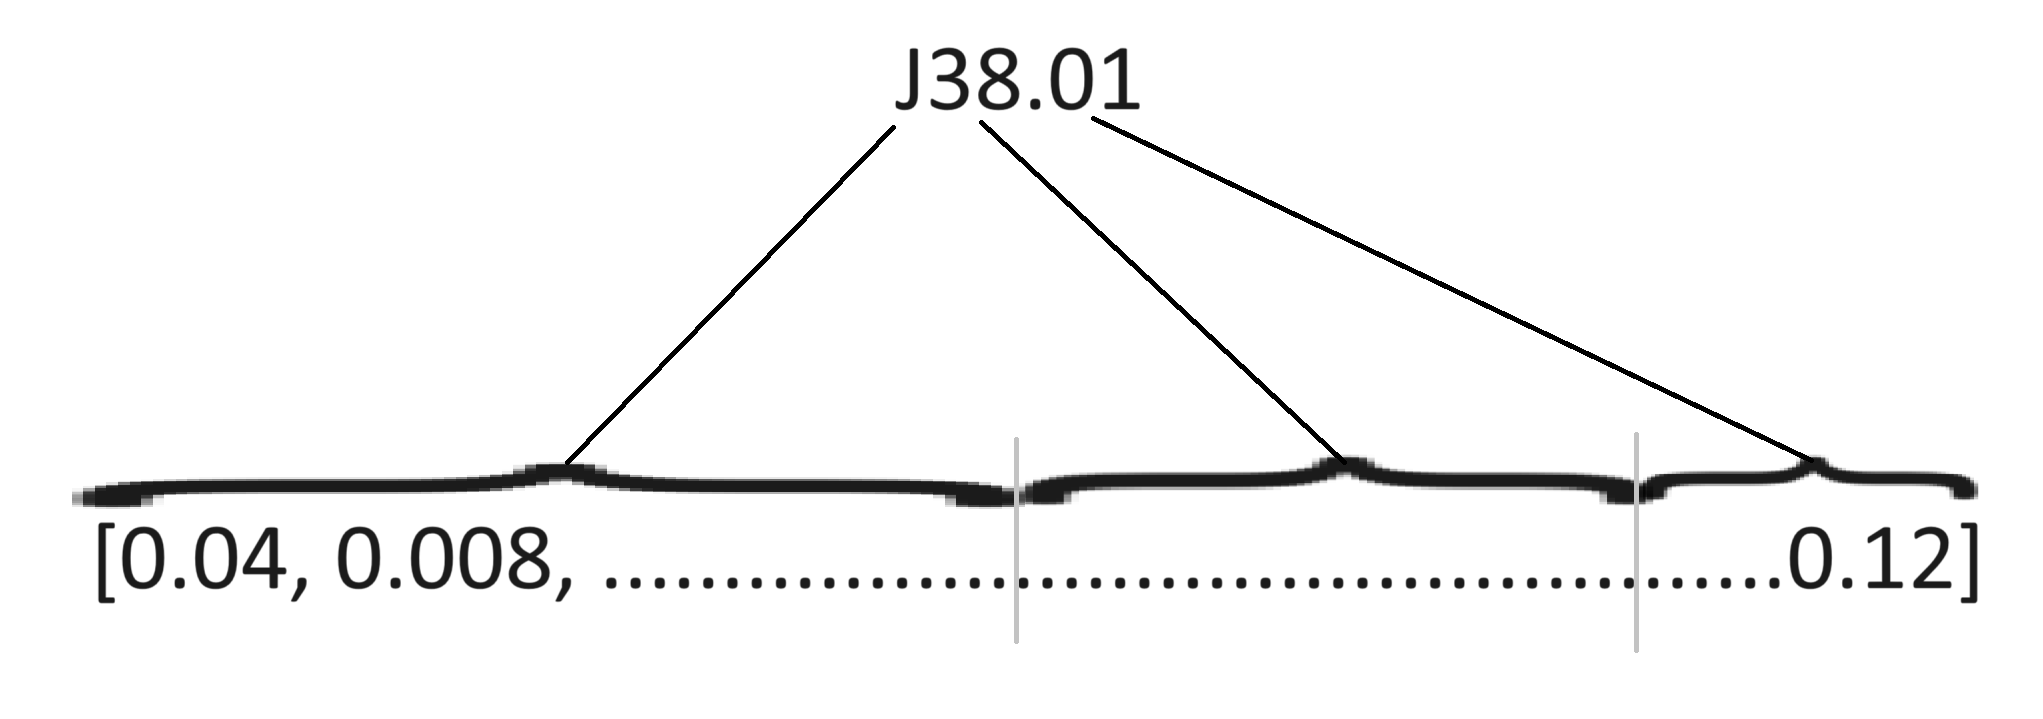
\includegraphics[height=2cm]{images/ICD_code_emb.png}
	\end{center}
\end{frame}

\subsection{Lieky}

\begin{frame}
	\frametitle{Lieky}
	\begin{itemize}
		\item<1> ATC kód
	\end{itemize}
	\begin{center}
		
\includegraphics[height=0.7cm]{images/ATC_code.png}
	\end{center}
	\begin{itemize}
		\item<1> N - Centrálna nervová sústava
		\item<1> N02 - Analgetiká
		\item<1> N02B - Iné analgetiká a antipyretiká
		\item<1> N02BA - Kyselina salicylová a deriváty
		\item<1> N02BA01 - Acylpyrín
	\end{itemize}
	
\end{frame}

\section{Ďalšie kroky}

\begin{frame}
	\frametitle{Ďalšie kroky}
	\begin{itemize}
		\item<1> vektorizácia celého záznamu pacienta
		\item<1> vytvorenie časového radu záznamov pre pacienta
		\item<1> návrh modelu (neurónovej siete)
		\item<1> nastavovanie a trénovanie modelu
		\item<1> validácia a hodnotenie modelu
	\end{itemize}
	
	
\end{frame}


\end{document}
